\documentclass[11pt]{article}

\usepackage[spanish,activeacute]{babel}
\usepackage{titlesec}
\usepackage{graphicx}
\usepackage{float}
\usepackage{subfig}
\usepackage{chngcntr}
\usepackage{xcolor}
\usepackage{listofitems}
\usepackage[bottom]{footmisc}
\usepackage[hidelinks]{hyperref}
\usepackage[most]{tcolorbox}


\setlength{\parindent}{1.0em}
\setlength{\parskip}{1.0em}
\setlength{\emergencystretch}{5.0em}
\setlength{\belowcaptionskip}{-10pt}
\counterwithin{figure}{section}
\titlespacing*{\section}{0em}{3.5em}{1.5em}
\setcounter{tocdepth}{2}
\hypersetup{
	linktoc=all
}


\title{\Huge Software en formato fuente}
\author{Eugenia Damonte, Ariel Fideleff y Mart\'in Go\~ni}
\date{}

\definecolor{fuchsia-vim}{RGB}{168,0,168}
\definecolor{orange-desert-vim}{RGB}{168,87,0}
\definecolor{darkgray}{RGB}{100,100,100}
\definecolor{light-blue}{RGB}{64, 76, 201}
\definecolor{light-red}{RGB}{201, 60, 60}
\definecolor{light-green}{RGB}{65, 181, 104}

\newtcolorbox{code-box}{colback=white!75!gray,colframe=white!15!gray,fontupper=\linespread{1.1}\selectfont}

\newcommand{\codetext}[2]{\large\texttt{\textcolor{#1}{#2}}}
\newcommand{\imagecaption}[1]{\vspace{-7pt}\caption*{\char91\ref{fig:#1}\char93}}


\begin{document}
	\pagenumbering{gobble}
	\maketitle
	\newpage
	\tableofcontents
	\newpage
	\pagenumbering{arabic}
	
	
	\section{Configuraci\'on previa}
		Antes de comenzar a resolver los ejercicios configuramos \texttt{vim} para editar archivos en C. Para hacer esto abrimos el archivo \texttt{\textasciitilde/.vimrc} (en todo caso de no existir, hay que crearlo) que es el archivo de configuraci'on de \texttt{vim}. Estaba vac'io por lo que le le a'nad'imos dos l'ineas: \texttt{set nocp} y \texttt{filetype plugin on}. Lo que hace el primer comando es desactivar el modo de compatibilidad. 'Este hace que algunas de las funciones de \texttt{vim} sean deshabilitadas o modificadas para que se comporte de manera similar a \texttt{vi}, el antecesor de \texttt{vim}. La segunda permite utlizar el plugin \texttt{filetype}.
		
		Luego para asegurarnos de tener todos los paquetes de \texttt{vim} utlizamos el comando \texttt{sudo apt-get install vim-gui-common vim-runtime}. El primer paquete tuvo que instalarse demorando varios minutos por la velocidad de descarga abismal de los repositorios. El segundo, por el otro lado ya estaba instalado en nuestro caso.
		
		Finalmente creamos el archivo de configuraci'on para los archivos con extensi'on \texttt{.c}, llamado \texttt{c.vim}. Para poder crearlo primero tuvimos que crear la carpeta \texttt{\textasciitilde/.vim/ftplugin}, que es donde se ponen los archivos de configuraci'on. Luego abrimos el mismo con \texttt{vim} y escribimos las configuraciones que quer'iamos usar.
		
		
		\begin{figure}[H]
			\centering
			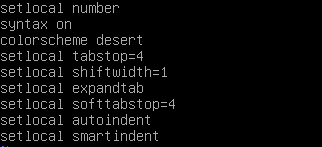
\includegraphics[width=.7\linewidth]{Images/Preamble/Preamble.PNG}
			\caption{Las configuraciones para los archivos \texttt{.c}}
			\label{fig:vim-setup}
		\end{figure}
		
		
	\section{Uso b'asico de gcc}
		Antes de comenzar con el proyecto en s'i, decidimos asegurarnos de que \texttt{gcc} funcionaba correctamente y que sab'iamos usarlo. Para hacer esto copiamos el programa de ejemplo, \texttt{circulo.c}, que se encuentra en el apunte provisto.
		
		\begin{figure}[H]
			\centering
			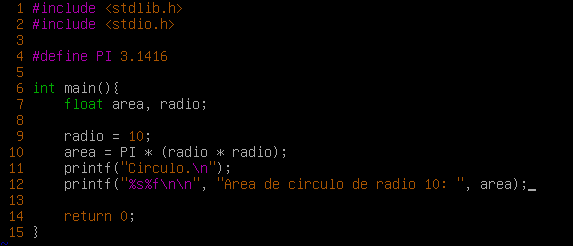
\includegraphics[width=.9\linewidth]{Images/Seccion 1/S1}
			\caption{El programa de ejemplo \texttt{circulo.c}}
		\end{figure}
		
	\subsection{Compilaci'on directa}
		Una vez copiado el programa realizamos una compilaci'on directa para asegurarnos de que el programa funcionase correctamente. Para hacer esto usamos el comando \texttt{gcc -o circulo circulo.c}. Lo que hace el argumento \texttt{-o} es permitirnos especificar el nombre delarchivo de salida, pues si no, el archivo se nombra por defecto \texttt{a.out}.
		
		\begin{figure}[H]
			\centering
			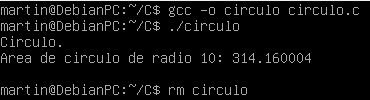
\includegraphics[width=.7\linewidth]{Images/Seccion 1/S1 parte dos}
			\caption{Muestra del funcionamiento de \texttt{circulo.c}}
			\label{fig:basic-compilation}
		\end{figure}
		
	\subsection{Compilaci'on compleja}
		Habiendo comprobado que \texttt{gcc} funcionaba correctamente decidimos intentar compilar el mismo archivo, \texttt{circulo.c}, de manera compleja. Es decir, haciendo cada uno de los pasos que realiza el compilador a la hora de transformar un archivo en C en un programa ejecutable, manualmente uno por uno.
	
	\subsubsection{Preprocesamiento}
		El preprocesado o preprocesamiento es la primera etapa de modificaci'on del c'odigo fuente. Sirve para que, en la fase de compilaci'on, que es la siguiente, el compilador pueda leer correctamente el c'odigo. 
    
    	El trabajo del preprocesador consiste en llevar a cabo las instrucciones dadas por las \textit{directivas} dirigidas al mismo (que, en el caso de C y C++, son las que comienzan con un numeral, como \texttt{\textcolor{fuchsia-vim}{\#define}}, \texttt{\textcolor{fuchsia-vim}{\#include}}, \texttt{\textcolor{fuchsia-vim}{\#ifdef}} y \texttt{\textcolor{fuchsia-vim}{\#error}}, entre otros).

   		En el archivo \texttt{circulo.c} podemos encontrar la directiva  \texttt{\textcolor{fuchsia-vim}{\#define PI} \textcolor{orange-desert-vim}{3.1416}}, que justamente define una constante de nombre \texttt{\textcolor{fuchsia-vim}{PI}} y valor \texttt{\textcolor{orange-desert-vim}{3.1416}}. Esta constante es llamada en la funci'on \texttt{main} de manera que, en vez de escribir  \texttt{\textcolor{orange-desert-vim}{3.1416}}, escribimos simplemente  \texttt{\textcolor{fuchsia-vim}{PI}}.

    	En la figura \ref{fig:preproc_circ},
   		se observa el c'odigo preprocesado que obtuvimos como salida del comando \texttt{gcc -E circulo.c} (tambi'en se puede usar \texttt{cpp circulo.c}, que hace referencia directamente al preprocesador). Si prestamos atenci'on, la directiva antes mencionada no figura en esta salida. Adem'as, en la l'inea que en el c'odigo fuente dec'ia \texttt{\textcolor{darkgray}{area = PI * (radio * radio)}}, ahora dice \texttt{\textcolor{darkgray}{area = \textcolor{orange-desert-vim}{3.1416} * (radio * radio)}}. 

   		En resumen, lo que hizo el preprocesador fue tomar esa definici'on que le indicamos en la directiva y coloc'o el valor de la constante en las partes del c'odigo en donde se hac'ia referencia a ella.
   		
   		\begin{figure}[H]
   			\centering
			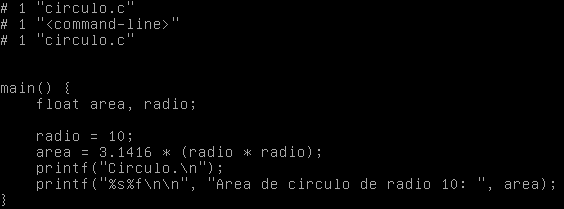
\includegraphics[width=.9\linewidth]{Images/Seccion 1/preprocesado_circulo}
   			\caption{Resultado del preprocesado de \texttt{circulo.c}}
   			\label{fig:preproc_circ}
   		\end{figure}

	\subsubsection{Compilaci'on}
		La compilaci'on es el proceso donde se transforma el c'odigo antes preprocesado (en nuestro caso en C), a assembler propio del procesador de la computadora (en espa'nol, \textit{lenguaje ensamblador}). Para hacer esto usamos el comando \texttt{gcc -S circulo.c}. Notar que directamente nos referimos al archivo con el c'odigo fuente \texttt{circulo.c}, pues el argumento \texttt{-S} ya de por medio realiza el preprocesado antes explicado. Finalmente verificamos que haya funcionado el comando, mostrando las primeras l'ineas del archivo \texttt{circulo.s}, que es donde \texttt{gcc} almacena el compilado.

		\begin{figure}[H]
			\centering
			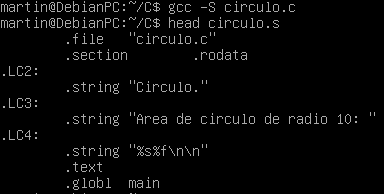
\includegraphics[width=.7\linewidth]{Images/Seccion 1/S1 parte tres.PNG}
			\caption{Primeras 10 l'ineas del resultado de la compilaci'on}
			\label{fig:complex-compilation}
		\end{figure}
		
	\subsubsection{Ensamblado}
		Una vez realizado el compilado, procedemos a ensamblar el archivo. Es decir, transformar el archivo de assembler a c'odigo objeto, un archivo binario en lenguaje m'aquina. Hicimos esto con el comando \texttt{as -o circulo.o circulo.s}. Luego verificamos que haya funcionado revisando qu'e tipo de archivo era \texttt{circulo.o} haciendo uso del comando \texttt{file}.
		
		Aclarar que otra forma por la cual podr'iamos haber obtenido el archivo en cuesti'on ser'ia el comando \texttt{gcc -c circulo.c}, pero como se puede ver, toma directamente desde el c'odigo fuente, ya que adem'as realiza todas las etapas previas explicadas.
		
		\begin{figure}[H]
			\centering
			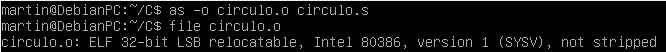
\includegraphics[width=.9\linewidth]{Images/Seccion 1/S1 parte cuatro}
			\caption{Ejecuci'on del ensamblado y detalles del archivo generado}
			\label{fig:complex-assembly}
		\end{figure}
	
		Al estar el archivo conseguido en lenguaje m'aquina, no es texto en s'i que podamos ver con facilidad. En todo caso, podemos hacer uso de un comando como lo es \texttt{objdump -d circulo.o}, que intepreta y permite ver las instrucciones a la computadora contenidas en el archivo. Hay que aclarar que las posiciones de memoria a las que se refiere probablemente no sean correctas, ya que 'estas deben ser relacionadas en el pr'oximo paso, el enlazado, con las librer'ias externas utilizadas.
		
	\subsubsection{Enlazado}
		Finalmente enlazamos el archivo. El enlazado es el proceso mediante el cual se vincula y se incorpora al programa, las librerias que requiere para poder funcionar. Estas librerias est'an compuestas de c'odigo con funciones que uno utiliza en dicho programa. Por ejemplo, en \texttt{circulo.c} usamos funciones como \texttt{\textcolor{darkgray}{printf}}, el cual hace referencia a la libreria \texttt{stdio.h} (t'ipicamente se definir'ia al comienzo del programa de la forma \texttt{\textcolor{fuchsia-vim}{\#include}\textcolor{orange-desert-vim}{\char60stdio.h\char62}} pero, al ser com'unmente utilizado, es incorporado autom'aticamente por el compilador).
		
		En este paso es donde nos encontramos con problemas. El comando que se da en el apunte no funciona. Al usarlo da varios errores indicando que las librerias usadas como argumentos no existen, as'i como tambi'en con algunas de las opciones del comando.
	
		\begin{figure}[H]
			\centering
			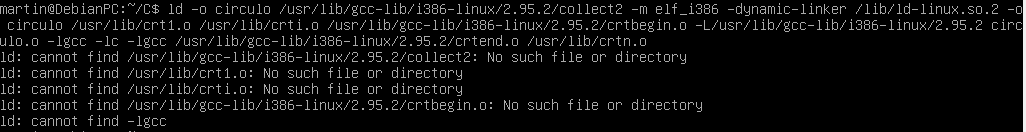
\includegraphics[width=.9\linewidth]{Images/Seccion 1/S1 parte cinco}
			\caption{El primer intento de usar \texttt{ld}, siguiendo el apunte}
			\label{fig:first-ld-attempt}
		\end{figure}
		
		Dado todos los errores que hab'ian, decidimos borrar todas las opciones innecesarias y probar nuevamente. Al hacer esto, los errores anteriores desaparecieron a cambio de uno nuevo. 'Este dec'ia ``\texttt{cannot find entry symbol \textunderscore\/start}'', el cual se traduce como ``\texttt{no se encuentra el simbolo de entrada \textunderscore\/start}''. Luego de algo de investigar descubrimos que este error se debe a que el verdadero punto de entrada\footnotemark\/ de un programa es \texttt{\textunderscore\/start} y no \texttt{main}, siendo que \texttt{\textunderscore\/start} simplemente redirige a 'el. Para solucionar esto usamos el argumento \texttt{--entry main} para especificar la funci'on \texttt{main} como el punto de entrada del programa.
		
		\footnotetext{El punto de entrada de un programa es donde se ejecutan las primeras instrucciones y se pasa control al programa.}
		
		Una vez hechos estos cambios la funci'on no daba mas errores y el programa parec'ia estar listo para usar. A la hora de ejecutarlo, sin embargo, 'este no era reconocido como un programa ejecutable. Para asegurarnos de haber hecho todo correctamente revisamos que el archivo existiese as'i como tambi'en sus permisos, siendo 'estos correctos.
		
		\begin{figure}[H]
			\centering
			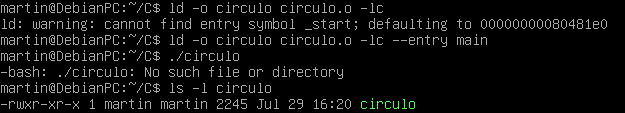
\includegraphics[width=.9\linewidth]{Images/Seccion 1/S1 parte seis}
			\caption{El segundo intento de usar \texttt{ld}}
			\label{fig:second-ld-attempt}
		\end{figure}
		
		Dado que no pod'iamos ejecutar el programa decidimos intentar volver a a'nadir algunas de las opciones que no causaban ores. Primero volvimos a a'nadir las opciones \texttt{-m elf\textunderscore\/i386} y \texttt{--dynamic-linker /lib/ld-linux.so.2}. La primera opci'on define el objetivo del compilador\footnotemark. La segunda define la ubicaci'on del enlazador din'amico\footnotemark\/ a usar.
		
		\footnotetext{El objetivo del compilador es lo que determina que tipo de c'odigo objeto debe producir la funci'on.}
		\footnotetext{Un enlazador din'amico o \textit{dynamic linker} es una forma de enlazar los archivos binarios que se necesitan para que el programa funcione. En este caso el c'odigo de las funciones se mantienen en la biblioteca y la hora de ejecutar el programa se cargan en memoria.}
		
		Luego de hacer estos cambios logramos ejecutar el programa, que parec'ia funcionar correctamente. Sin embargo, al final de 'este tuvimos el error \texttt{Segmentation fault}. Para tratar de averiguar de donde ven'ia el error decidimos debuggear el programa utilizando \texttt{gdb}.
		
		\begin{figure}[H]
			\centering
			\subfloat[Error al correr el programa]{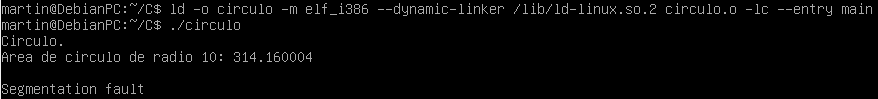
\includegraphics[width=.8\linewidth]{Images/Seccion 1/S1 parte siete}} \par
			\subfloat[Nuestro intento de debuggear el programa]{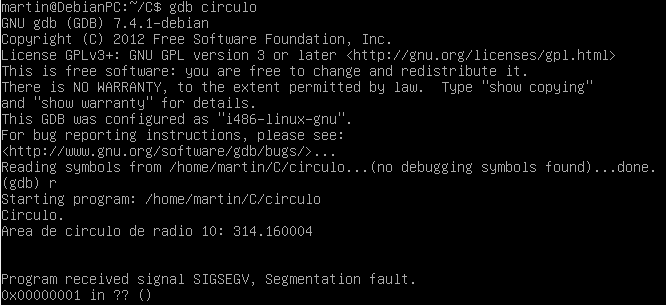
\includegraphics[width=.8\linewidth]{Images/Seccion 1/S1 parte ocho}}
			
			\caption{El tercer intento de usar \texttt{ld}}
			\label{fig:third-ld-attempt}
		\end{figure}
		
		Cuando intentamos debuggear el programa nos encontramos con algo extra'no, y es que \texttt{gdb} no sab'ia de qu'e l'inea proven'ia el error. Esto nos llev'o a creer que proven'ia del enlazado del programa, y no del programa en s'i. Luego de buscar m'as todav'ia, encontramos el problema, y es que nos faltaba incluir las librerias que requer'ia el enlazador din'amico. Para entender por qu'e pasa esto hay que entender c'omo funciona el comando.
		
		Lo primero que hace el comando es especificar la ubicaci'on del enlazador din'amico que requieren las dem'as librerias para acceder a las funciones din'amicas de C. Luego se incluyen otras tres librerias \texttt{/usr/lib/i386-linux-gnu/crt1.o}, \texttt{/usr/lib/i386-linux-gnu/crti.o} y \texttt{/usr/lib/i386-linux-gnu/crtn.o}. La primera es la librer'ia que tiene referencias a los archivos que requiere el enlazador (\texttt{/lib/libc.so.6} y \texttt{/usr/lib/libc\textunderscore\/nonshared.a}). Las otras dos se encargan de que existan \texttt{\textunderscore\/init} y \texttt{\textunderscore\/fini}, que son el c'odigo de inicializaci'on y finalizaci'on. Algo importante de recordar es que la ubicaci'on de las librerias puede cambiar dependiendo del sistema y la instalaci'on especifica. En nuestro caso, las encontramos buscando en \texttt{/usr/lib} y revisando todas las carpetas que parec'ian tener alguna relaci'on.
	
		Es importante notar la posici'on de las librer'ias, \texttt{crti.o} debe ir despu'es de \texttt{crt1.o}. Esto es porque el segundo hace referencia al primero. Adem'as ambas deben ir antes del archivo que se est'a enlazando. Finalmente \texttt{crtn.o} va al final del comando, despu'es de todos los dem'as argumentos.
		
		\begin{figure}[H]
			\centering
			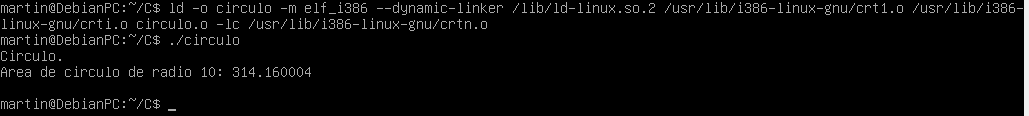
\includegraphics[width=.9\linewidth]{Images/Seccion 1/S1 parte nueve.PNG}
			\caption{El cuarto y 'ultimo intento de usar \texttt{ld}}
			\label{fig:fourth-ld-attempt}
		\end{figure}
		
		Luego de hacer todo esto, el programa finalmente funcion'o y se ejecut'o de manera correcta y sin errores. Habiendo terminado decidimos que ya ten'iamos el suficiente conocimiento para intentar compilar un programa usando \texttt{make}.
		
	\section{Comandos usados}
		A continuaci'on se encuentran todos los comandos utilizados en este trabajo, correspondientes a las im'agenes presentadas.
		
		\begin{figure}[H]
			\centering
			\begin{code-box}
				\codetext{light-blue}{setlocal} \codetext{light-red}{number}
				
				\codetext{light-blue}{syntax} \codetext{light-red}{on}

				\codetext{light-blue}{colorscheme} \codetext{light-red}{desert}
				
				\codetext{light-blue}{setlocal} \codetext{light-red}{tabstop=4}

				\codetext{light-blue}{setlocal} \codetext{light-red}{shiftwidth=1}
				
				\codetext{light-blue}{setlocal} \codetext{light-red}{expandtab}
				
				\codetext{light-blue}{setlocal} \codetext{light-red}{softtabstop=4}
				
				\codetext{light-blue}{setlocal} \codetext{light-red}{autdoindent}
				
				\codetext{light-blue}{setlocal} \codetext{light-red}{smartindent}
			\end{code-box}
			\imagecaption{vim-setup}
		\end{figure}
		
		\begin{figure}[H]
			\centering
			\begin{code-box}
				\codetext{light-blue}{gcc} \codetext{orange-desert-vim}{-o circulo} \codetext{light-red}{circulo.c}
				
				\codetext{light-blue}{./circulo}
				
				\codetext{light-blue}{rm} \codetext{light-red}{circulo}
			\end{code-box}
			\imagecaption{basic-compilation}
		\end{figure}
		
		\begin{figure}[H]
			\centering
			\begin{code-box}
				\codetext{light-blue}{gcc} \codetext{orange-desert-vim}{-S} \codetext{light-red}{circulo.c}
				
				\codetext{light-blue}{head} \codetext{light-red}{circulo.s}
			\end{code-box}
			\imagecaption{complex-compilation}
		\end{figure}
		
		\begin{figure}[H]
			\centering
			\begin{code-box}
				\codetext{light-blue}{as} \codetext{orange-desert-vim}{-o circulo.o} \codetext{light-red}{circulo.s}
				
				\codetext{light-blue}{file} \codetext{light-red}{circulo.o}
			\end{code-box}
			\imagecaption{complex-assembly}
		\end{figure}
		
		\begin{figure}[H]
			\centering
			\begin{code-box}
			\codetext{light-blue}{ld} \codetext{orange-desert-vim}{-o circulo /usr/lib/gcc-lib/i386-linux/2.95.2/ collect2 -m elf\textunderscore{}i386 --dynamic-linker /lib/ld-linux.so.2 -o circulo /usr/lib/crt1.o /usr/lib/crti.o /usr/lib/gcc-lib/i386-linux/2.95.2/ crtbegin.o -L /usr/lib/gcc-lib/i386-linux/2.95.2} \codetext{light-red}{circulo.o }\codetext{orange-desert-vim}{-lgcc -lc -lgcc /usr/lib/gcc-lib/ i386-linux/2.95.2/crtend.o /usr/lib/crtn.o}
			\end{code-box}
			\imagecaption{first-ld-attempt}
		\end{figure}
		
		\begin{figure}[H]
			\centering
			\begin{code-box}
				\codetext{light-blue}{ld} \codetext{orange-desert-vim}{-o circulo} \codetext{light-red}{circulo.o} \codetext{orange-desert-vim}{-lc}
				
				\codetext{light-blue}{ld} \codetext{orange-desert-vim}{-o circulo} \codetext{light-red}{circulo.o} \codetext{orange-desert-vim}{-lc --entry main}
				
				\codetext{light-blue}{./circulo}
				
				\codetext{light-blue}{ld} \codetext{orange-desert-vim}{-l} \codetext{light-red}{circulo}
			\end{code-box}
			\imagecaption{second-ld-attempt}
		\end{figure}
		
		\begin{figure}[H]
			\centering
			\begin{code-box}
				\codetext{light-blue}{ld} \codetext{orange-desert-vim}{-o circulo -m elf\textunderscore\/i386 --dynamic-linker /lib/ld-linux.so.2} \codetext{light-red}{circulo.o} \codetext{orange-desert-vim}{-lc --entry main}
				
				\codetext{light-blue}{./circulo}
				
				\codetext{light-blue}{gdb} \codetext{light-red}{circulo}
				
				\codetext{light-green}{(gdb)} \codetext{light-blue}{r}
			\end{code-box}
			\imagecaption{third-ld-attempt}
		\end{figure}
		
		\begin{figure}[H]
			\centering
			\begin{code-box}
				\codetext{light-blue}{ld }\codetext{orange-desert-vim}{-o circulo -m elf\textunderscore\/i386 --dynamic-linker /lib/ld-linux.so.2 /usr/lib/i386-linux-gnu/ crt1.o /usr/lib/i386-linux-gnu/crti.o} \codetext{light-red}{circulo.o} \codetext{orange-desert-vim}{-lc /usr/lib/i386-linux-gnu/crtn.o}
				
				\codetext{light-blue}{./circulo}
			\end{code-box}
			\imagecaption{fourth-ld-attempt}
		\end{figure}
		
		
		
		
		
		
		
		
		
		
				

		


















%Remove whitspace when done, for ease of work.
\end{document}
